\chapter{Metodologia} \section*{Elementos do processamento e análise de imagem}
Os principais dispositivos de exibição usados nos modernos sistemas de
processamento de imagens são os monitores de televisão (TV), monocromáticos e
coloridos.  Além desses, incluem-se na lista dos equipamentos responsáveis pela
apresentação dos resultados das aquisições de imagens, os tubos de raios
catódicos e dispositivos de impressão \cite{LIM}. A Figura \ref{fig:elemProc}
apresenta o modelo proposto para um sistema de processamento e análise de
imagem.



\begin{figure}[ht] \centering 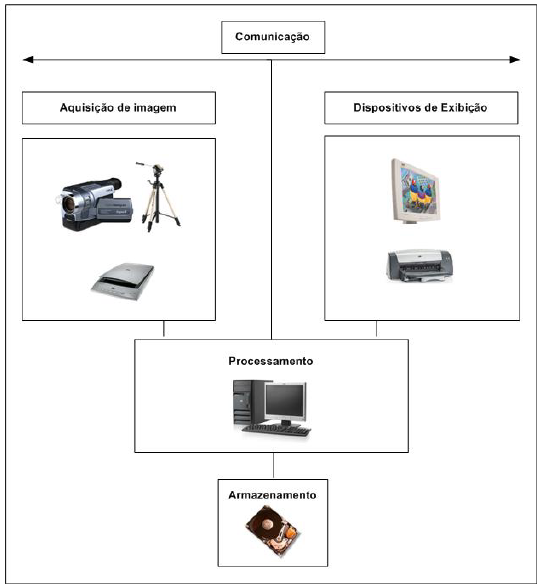
\includegraphics[scale=0.7]{figures/elemProc.png}
	\caption{Elementos do processamento e análise de imagem. Fonte: \cite{PACHECO} }
	\label{fig:elemProc} \end{figure}


\section*{Placa de prototipação alvo} A prototipação do sistema será realizada
utilizando com alvo a placa  XUPV5-LX110T, que posui o FPGA  XC5VLX110T da
família \textit{Virtex-5}. Além do FPGA a placa oferece diversos outros
recursos para aplicaçãoes avançadas, como rede giga-bit, porta sata,
\textit{usb-host}, processador \textit{ Open-Sparc}, dentre outros
\cite{XILINX}.  A placa também oferece estruturas de memória que serão
extremamente importantes para a concepção, visto que tanto o sistema
operacional e os módulos descritos em HDL farão uso da mesma.  
A Figura \ref{fig:placa} mostra os recursos que se pretende utilizar no estudo. Além dos 
recursos fornecidos pela placa também será necessário uma placa de captura usb e uma câmera.

\begin{figure}[ht] \centering 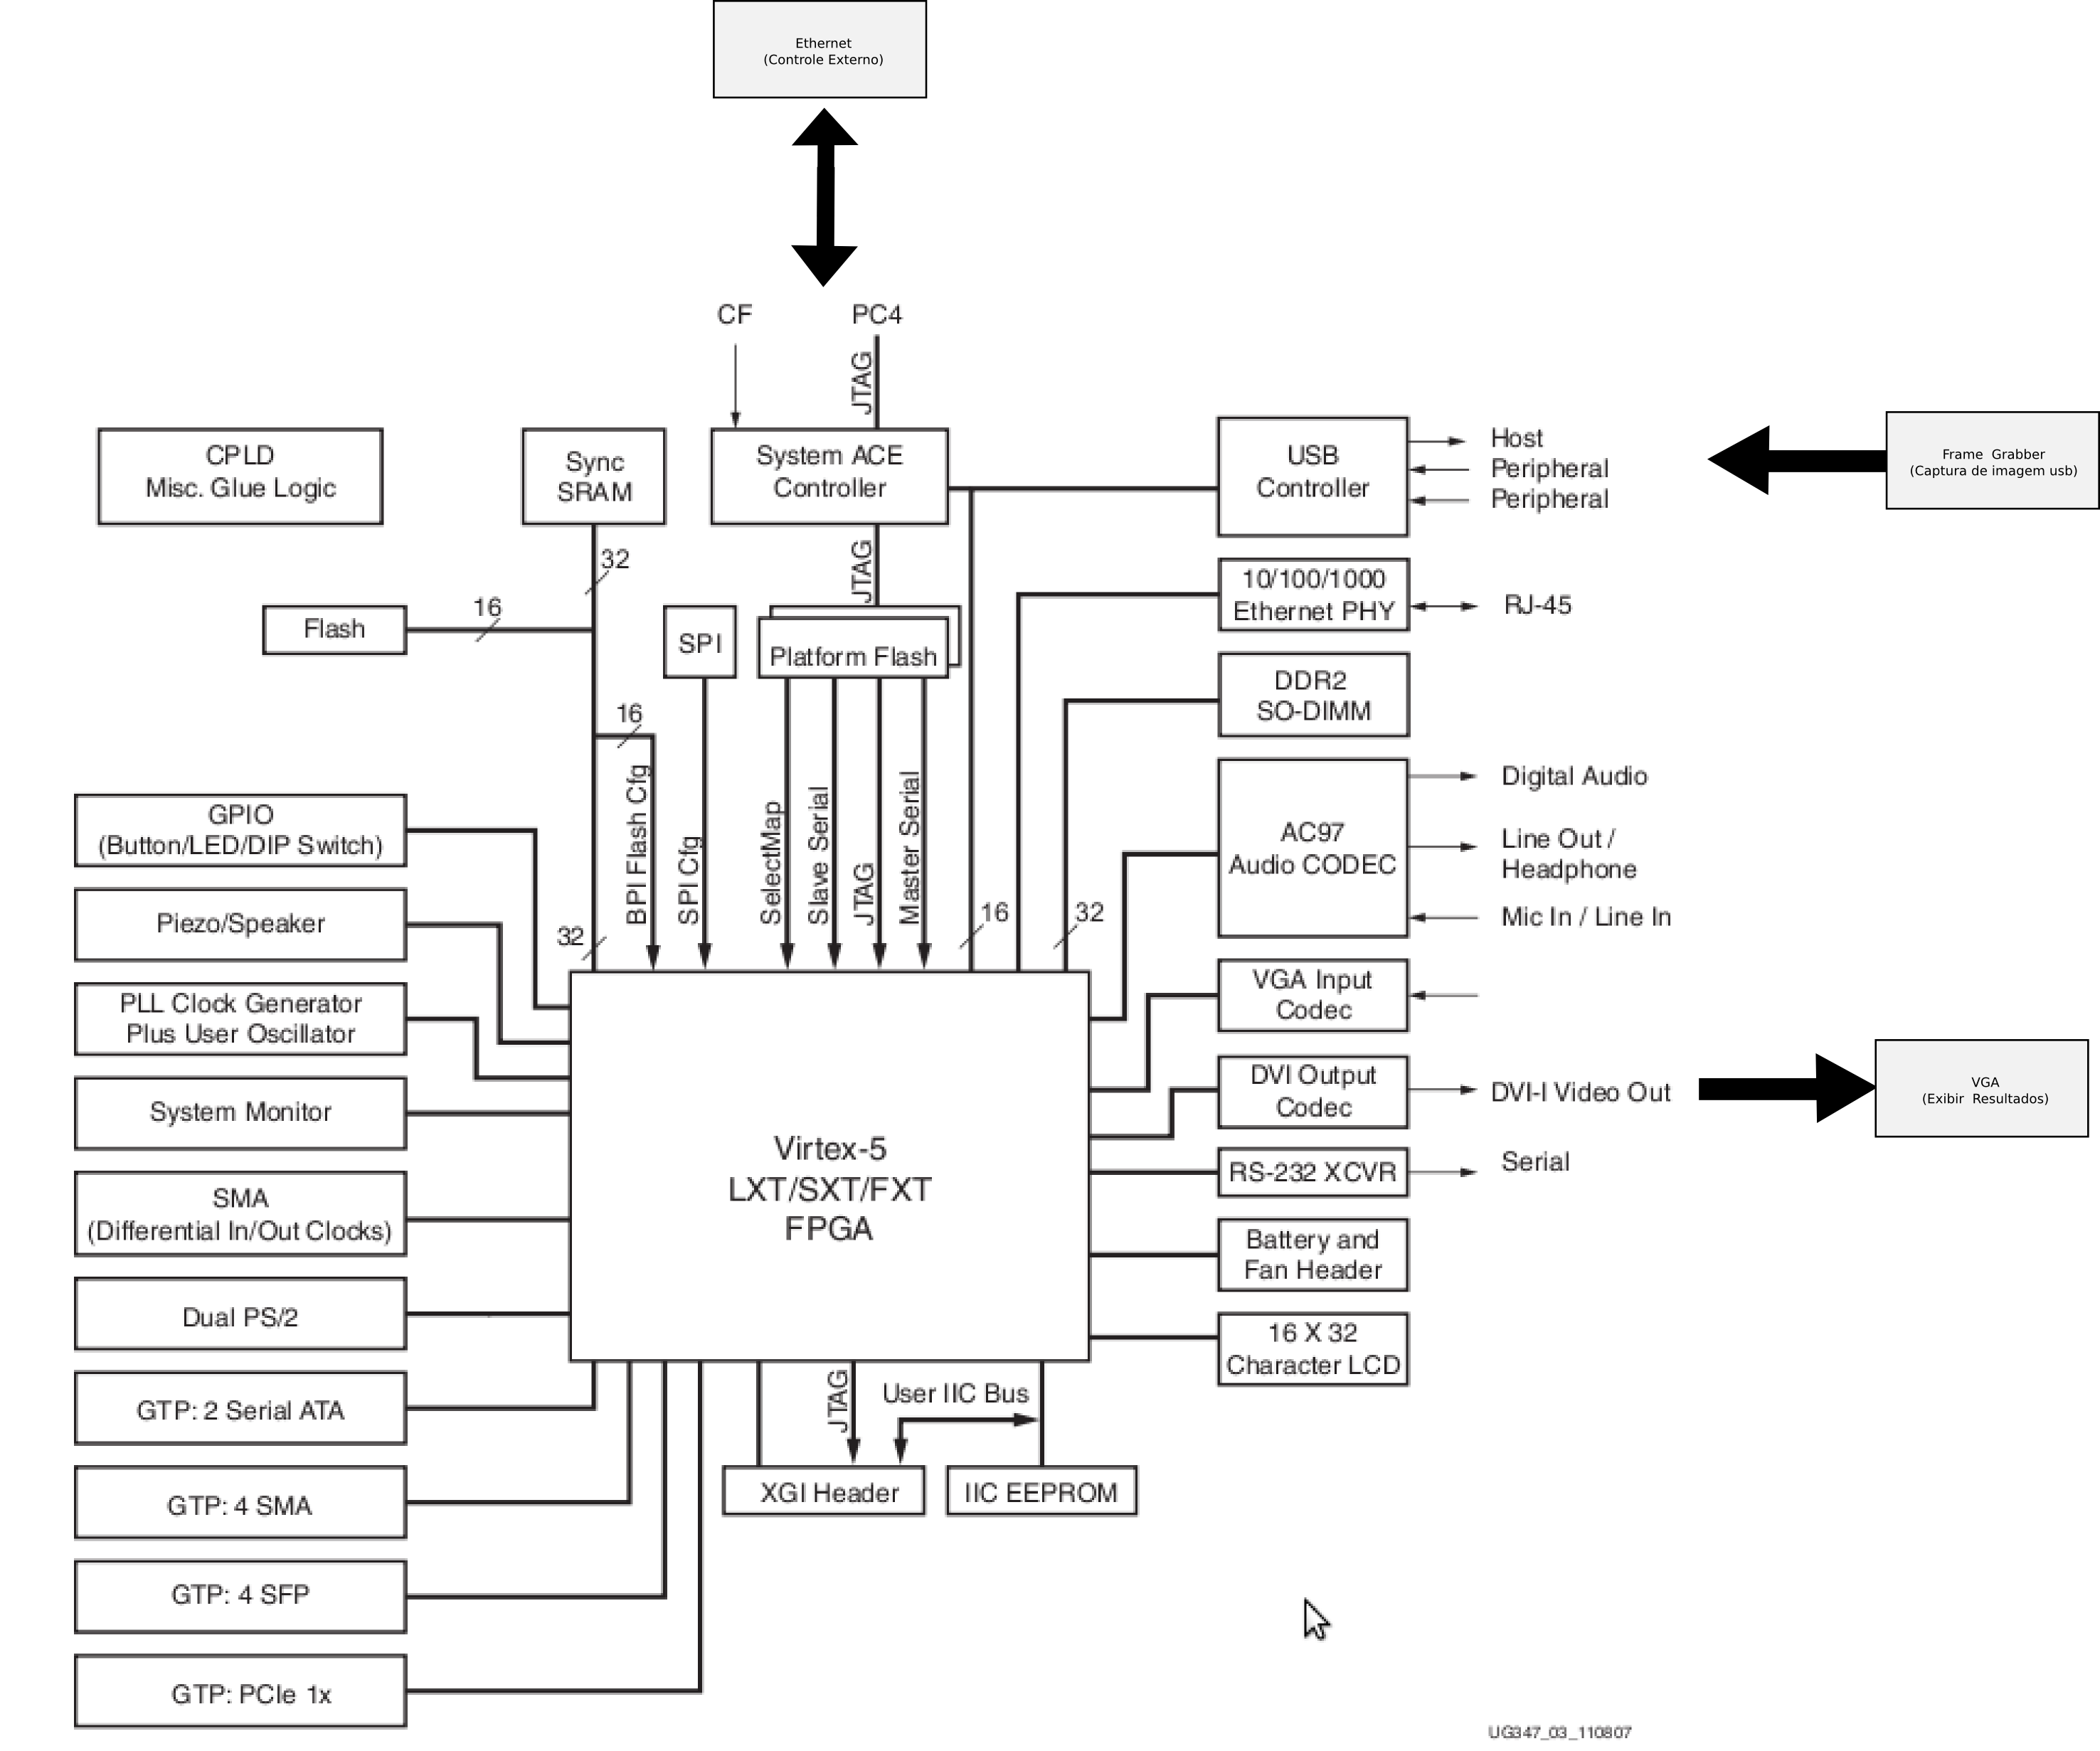
\includegraphics[scale=0.8]{figures/recursos.png}
	\caption{Plataforma de desenvolvimento Virtex-V , da \textit{Xilinx}.
	Fonte: \cite{XILINX}} \label{fig:placa} \end{figure}

\section*{Modelo Proposto} O objetivo deste estudo é criar um sistema
com base na implementação desenvolvida por Márcio Alexandre Pacheco, integrando a
etapa de captura de imagem e reconhecimento por redes neurais. 

\begin{figure}[ht] \centering 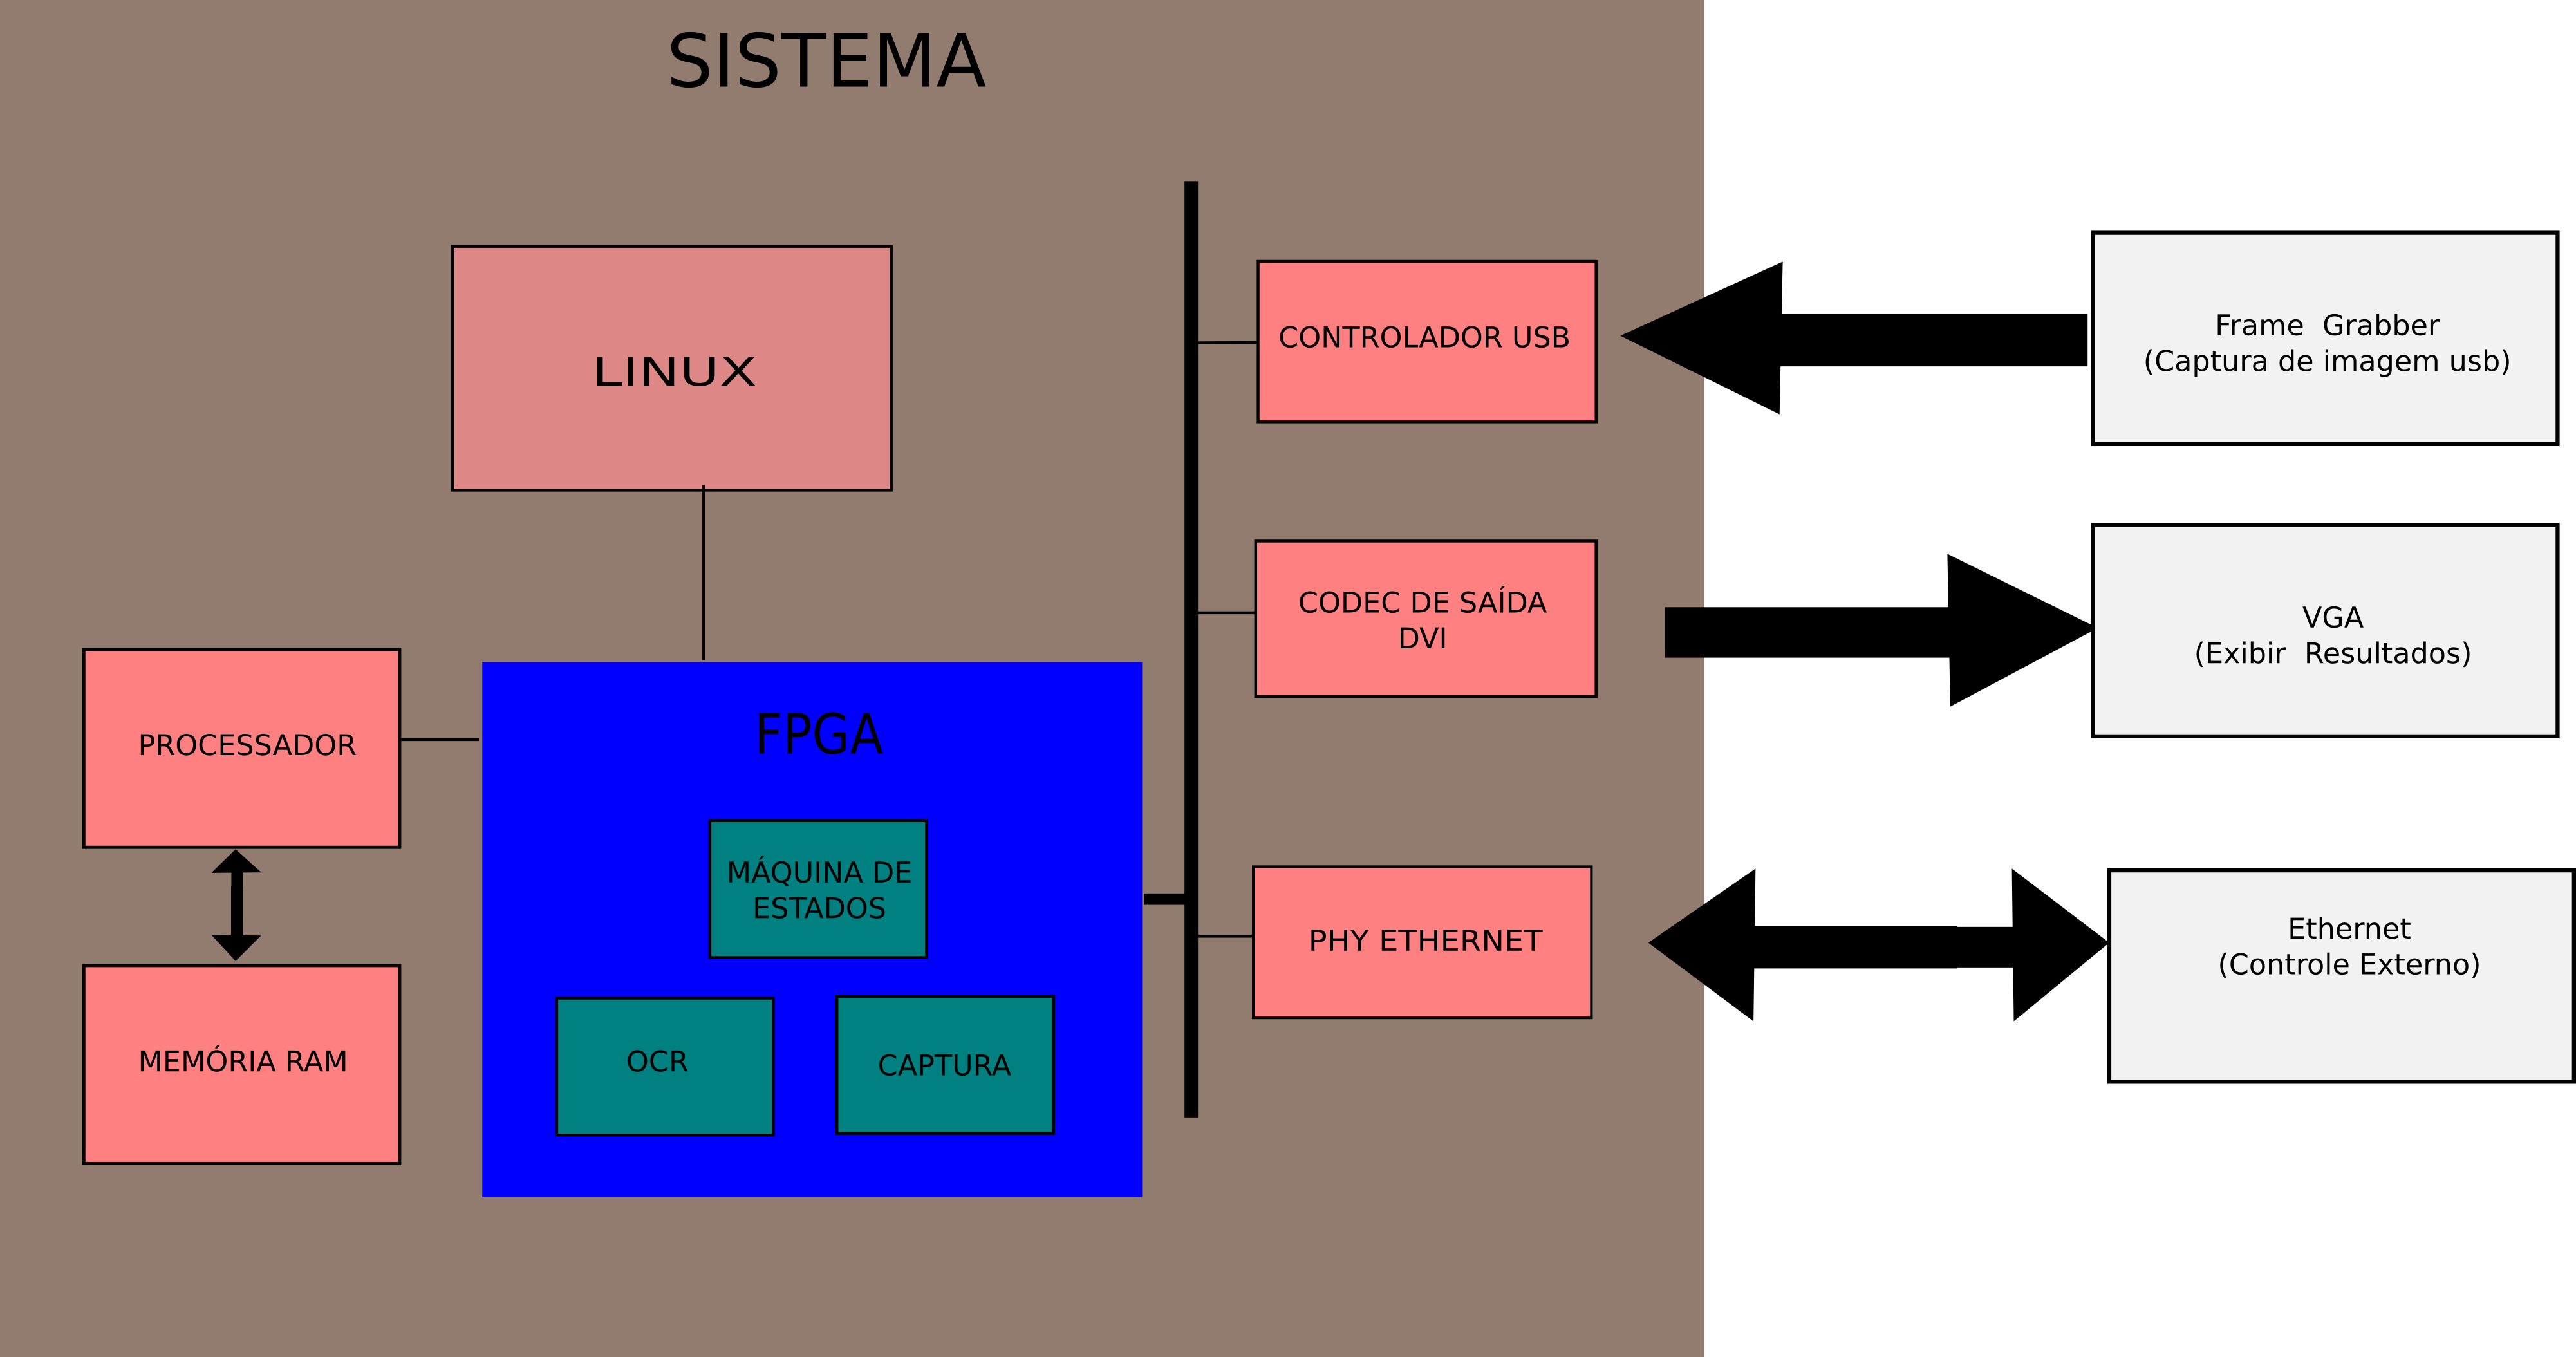
\includegraphics[scale=0.6]{figures/sis.png}
	\caption{Sistema Proposto} \label{fig:sisProp} \end{figure}

Dentro do FPGA estará a máquina de estados que fará o controle de toda a
análise de imagem, sendo iniciada através de um estimulo externo gerado por um
pino de IO. A imagem que será analisada será capturada por uma câmera acoplada
a um \textit{frame-grabber}, que é um dispositivo para captura de imagens pela
porta \textit{usb}.

A imagem será enviada através do barramento para o FPGA, que armazenará os
dados na memória. O FPGA consome os dados do modelo para obter o total de regiões
candidatas, extração e reconhecimento dos caracteres.  A
Figura \ref{fig:sisProp} mostra a arquitetura do dispositivo.

	\section*{Estratégia de validação do sistema a ser implementado} A
	validação do sistema será realizada com o método típico para validação
	de módulos em \textit{hardware} sendo comparado o desempenho em suas respectivas arquiteturas. 
  Após a integração de todos os módulos os resultados serão comparados ao OCR já implementado em PC e que 
  faz uso dos mesmos algoritmos de extração de regiões candidatas, extração de caracteres e reconhecimento através de redes neurais.
	
